%%%%%%%%%%%%%%%%%%%%%%%%%%%%%%%%%%%%%%
% LaTeX poster template
% Created by Nathaniel Johnston
% August 2009
% http://www.nathanieljohnston.com/2009/08/latex-poster-template/
%%%%%%%%%%%%%%%%%%%%%%%%%%%%%%%%%%%%%%

\documentclass[final, table]{beamer}
%\usepackage[scale=1.24]{beamerposter}
\usepackage[size=a1,scale=1.1]{beamerposter}
\usepackage{graphicx}			% allows us to import images
\usepackage{subfigure}

%-----------------------------------------------------------
% Define the column width and poster size
% To set effective sepwid, onecolwid and twocolwid values, first choose how many columns you want and how much separation you want between columns
% The separation I chose is 0.024 and I want 4 columns
% Then set onecolwid to be (1-(4+1)*0.024)/4 = 0.22
% Set twocolwid to be 2*onecolwid + sepwid = 0.464
%-----------------------------------------------------------

\newlength{\sepwid}
\newlength{\onecolwid}
\newlength{\twocolwid}
\newlength{\threecolwid}
\setlength{\paperwidth}{48in}
\setlength{\paperheight}{42in}
%\setlength{\paperwidth}{42in}
%\setlength{\paperheight}{36in}
\setlength{\sepwid}{0.024\paperwidth}
\setlength{\onecolwid}{0.22\paperwidth}  % For 4 columns
%\setlength{\onecolwid}{0.30\paperwidth}   % 3 columns
\setlength{\twocolwid}{0.464\paperwidth}
\setlength{\threecolwid}{0.708\paperwidth}
\setlength{\topmargin}{-0.5in}
\usetheme{confposter}
\usepackage{exscale}
\usepackage[font=singlespacing]{caption}
\usepackage{multirow}

%-----------------------------------------------------------
% The next part fixes a problem with figure numbering. Thanks Nishan!
% When including a figure in your poster, be sure that the commands are typed in the following order:
% \begin{figure}
% \includegraphics[...]{...}
% \caption{...}
% \end{figure}
% That is, put the \caption after the \includegraphics
%-----------------------------------------------------------

%\usecaptiontemplate{
%\small
%\structure{\insertcaptionname~\insertcaptionnumber:}
%\insertcaption}
\setbeamertemplate{caption}[numbered]

%-----------------------------------------------------------
% Define colours (see beamerthemeconfposter.sty to change these colour definitions)
%-----------------------------------------------------------

\setbeamercolor{block title}{fg=dblue,bg=white}
\setbeamercolor{block body}{fg=black,bg=white}
\setbeamercolor{block alerted title}{fg=white,bg=dblue!70}
\setbeamercolor{block alerted body}{fg=black,bg=dblue!10}

%-----------------------------------------------------------
% Math commands
%-----------------------------------------------------------
\newcommand{\X}{\mathcal{X}}
\newcommand{\Y}{\mathcal{Y}}
\newcommand{\G}{\mathcal{G}}
\newcommand{\norm}[1]{\left | \left | #1 \right | \right |}
\newcommand{\reals}{\mathbb{R}}
\newcommand{\scrF}{\mathcal{F}}
\newcommand{\E}{\mathbb{E}}
\newcommand{\K}{\mathcal{K}}
\newcommand{\PP}{\mathbb{P}}
\newcommand{\N}{\mathbb{N}}
\newcommand{\Dir}{\text{Dir}}
\newcommand{\DP}{\text{DP}}
\newcommand{\Pois}{\text{Pois}}
\newcommand{\BP}{\text{BP}}
\newcommand{\BeP}{\text{BeP}}
\newcommand{\borel}{\mathcal{B}}
\newcommand{\Beta}{\text{Beta}}
\newcommand{\Discrete}{\text{Discrete}}
\newcommand{\Ber}{\text{Bernoulli}}
\newcommand{\CRP}{\text{CRP}}
\newcommand{\IBP}{\text{IBP}}
\newcommand{\Norm}{\text{N}}
\newcommand{\B}{\mathcal{B}}
\newcommand{\Corr}{\text{Corr}}
\newcommand{\Un}{\text{Un}}
\newcommand{\CRM}{\text{CRM}}
\newcommand{\NiG}{\text{NiG}}
\newcommand{\Cat}{\text{Cat}}
\newcommand{\T}{\mathcal{T}}
\newcommand{\Ga}{\text{Ga}}
\newcommand{\notrightarrow}{\centernot\rightarrow}
\newcommand{\gap}{\text{    }}



%-----------------------------------------------------------
% Name and authors of poster/paper/research
%-----------------------------------------------------------

\title{An Array Tomography Exploration Tool: \\ \textit{Exploring Synapses from FMR1 Knockout Mice}}
\author{
Anish K. Simhal		\textsuperscript{1*},
Kristina D. Micheva		\textsuperscript{2}
Yi Zuo				\textsuperscript{3},
Richard J. Weinberg		\textsuperscript{4}, \\
Stephen J. Smith		\textsuperscript{5}, 
Guillermo Sapiro		\textsuperscript{1}}
\institute{\textsuperscript{1}Duke University 
\textsuperscript{2} Stanford University School of Medicine
\textsuperscript{3} University of California, Santa Cruz \\
\textsuperscript{4} University of North Carolina, Chapel Hill
\textsuperscript{5} Allen Institute for Brain Sciences }


%-----------------------------------------------------------
% Start the poster itself
%-----------------------------------------------------------
\begin{document} 
\addtobeamertemplate{headline}{} 
{\begin{tikzpicture}[remember picture, overlay]
\node [anchor=north west, inner sep=5cm]  at (current page.north west)
{
\includegraphics[scale=3.5]{figs/dukelogo}};
\end{tikzpicture}
\vspace{6cm} %twiddle with this later...
\begin{tikzpicture}[remember picture, overlay]
\node [anchor=north east, inner sep=4cm]  at (current page.north east)
{
\includegraphics[scale=0.55]{figs/IID_logo}};
\end{tikzpicture}
}
\begin{frame}[t]  
\begin{columns}[t]  % align column content at top

% First column
\begin{column}{\sepwid}\end{column}  % spacer column
\begin{column}{\onecolwid} 

\begin{block}{Overview} 

\begin{itemize}

\item Array tomography allows collection of data sets containing synaptic protein markers and markers for dendrites, axons, glial cells, nuclei, myelin, and mitochondria.

\item We here introduce the {\it Array Tomography Exploration Tool (ATET)}, a suite of computer vision methods that facilitate the exploration of array tomography data. 

\item We use array tomography and ATET to compare the relationship between astrocytes and synapses in the barrel cortex of a knockout mouse versus a wild-type mouse. 

\end{itemize}

\textbf{Fragile X syndrome} (FXS) is the most common form of genetically inherited mental retardation.  It is caused by the transcriptional silencing of the FMR1 gene that encodes the fragile X mental retardation protein. In this study, we used 4-month-old FMR1 knock out mice (a mouse model of FXS) and characterized synapses in the barrel cortex between FMR1$^{+/y}$ and FMR1$^{-/y}$ males.


\end{block}

\begin{block}{Array Tomography Pipeline} 

\begin{figure}
\centering
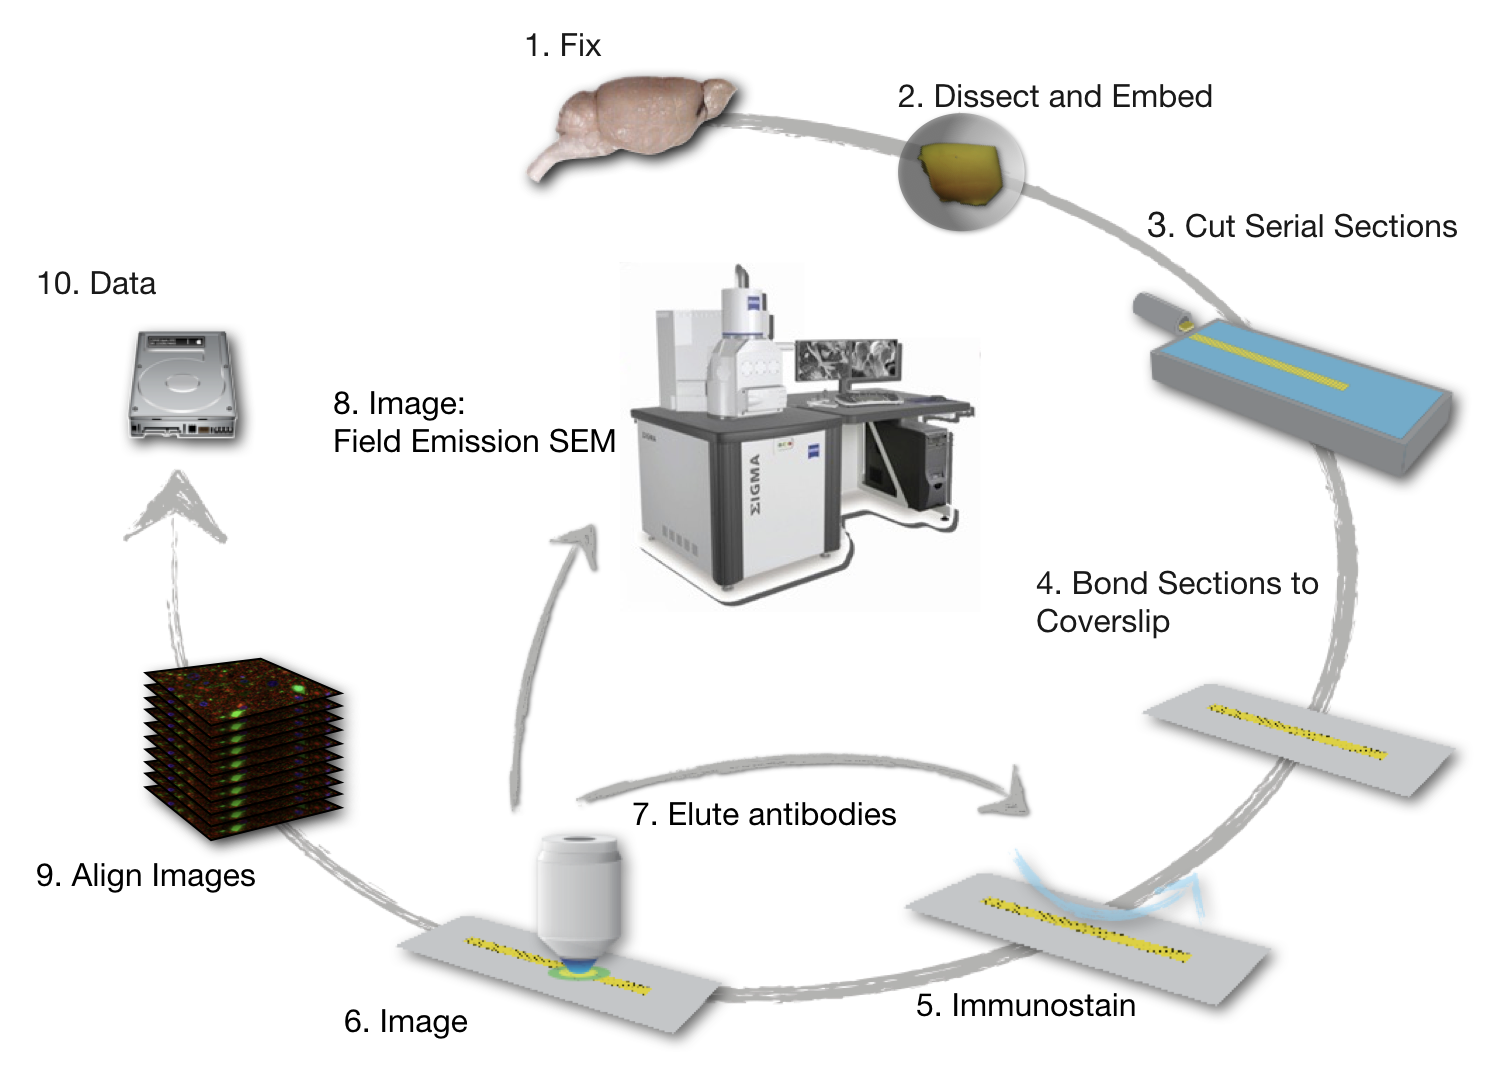
\includegraphics[width=0.9\textwidth]{figs/atpipeline}
\caption{\textit{Pipeline of the array tomography (AT) approach used for creating the data}}
\end{figure}

\begin{figure}
\centering
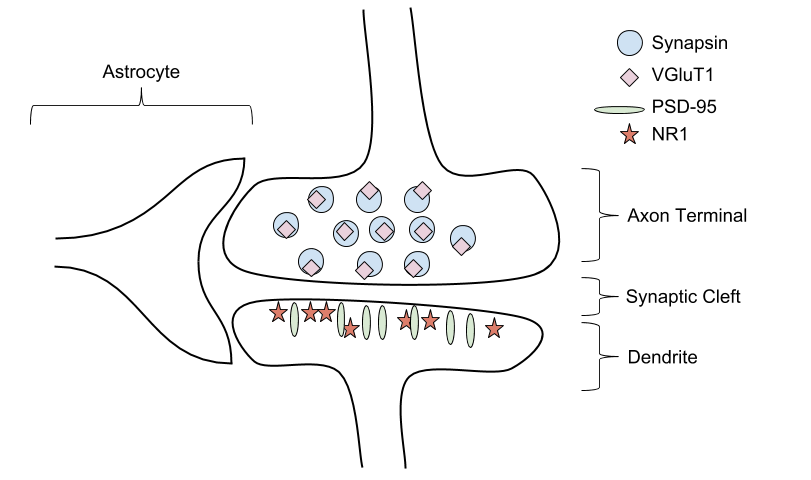
\includegraphics[width=0.8\textwidth]{figs/synapsecartoon}
\caption{\textit{Cartoon showing the relative spatial arrangement of the different parts of a tripartite synapse}}
\end{figure}

\end{block} 


\begin{block}{References}
\tiny{
\begin{thebibliography}{99}


\bibitem{Micheva2} 
Micheva KD, Smith SJ. Array tomography: a new tool for imaging the molecular architecture and ultrastructure of neural circuits. Neuron. 2007 Jul 5;55(1):25-36.

\bibitem{Simhal} 
Simhal, Anish K., et al. Probabilistic Fluorescence-Based Synapse Detection. PLoS Computational Biology, May 2017.

\bibitem{Simhal2} 
Simhal, Anish K., et al. A Computational Synaptic Antibody Characterization Tool for Array Tomography. Frontiers in Neuroanatomy. 2018;12.

\end{thebibliography}}
\end{block}








\end{column}

% Second column
\begin{column}{\sepwid}\end{column}  % spacer column
\begin{column}{\twocolwid}

\begin{block}{Array Tomography Exploration Tool}

\begin{figure}
\centering
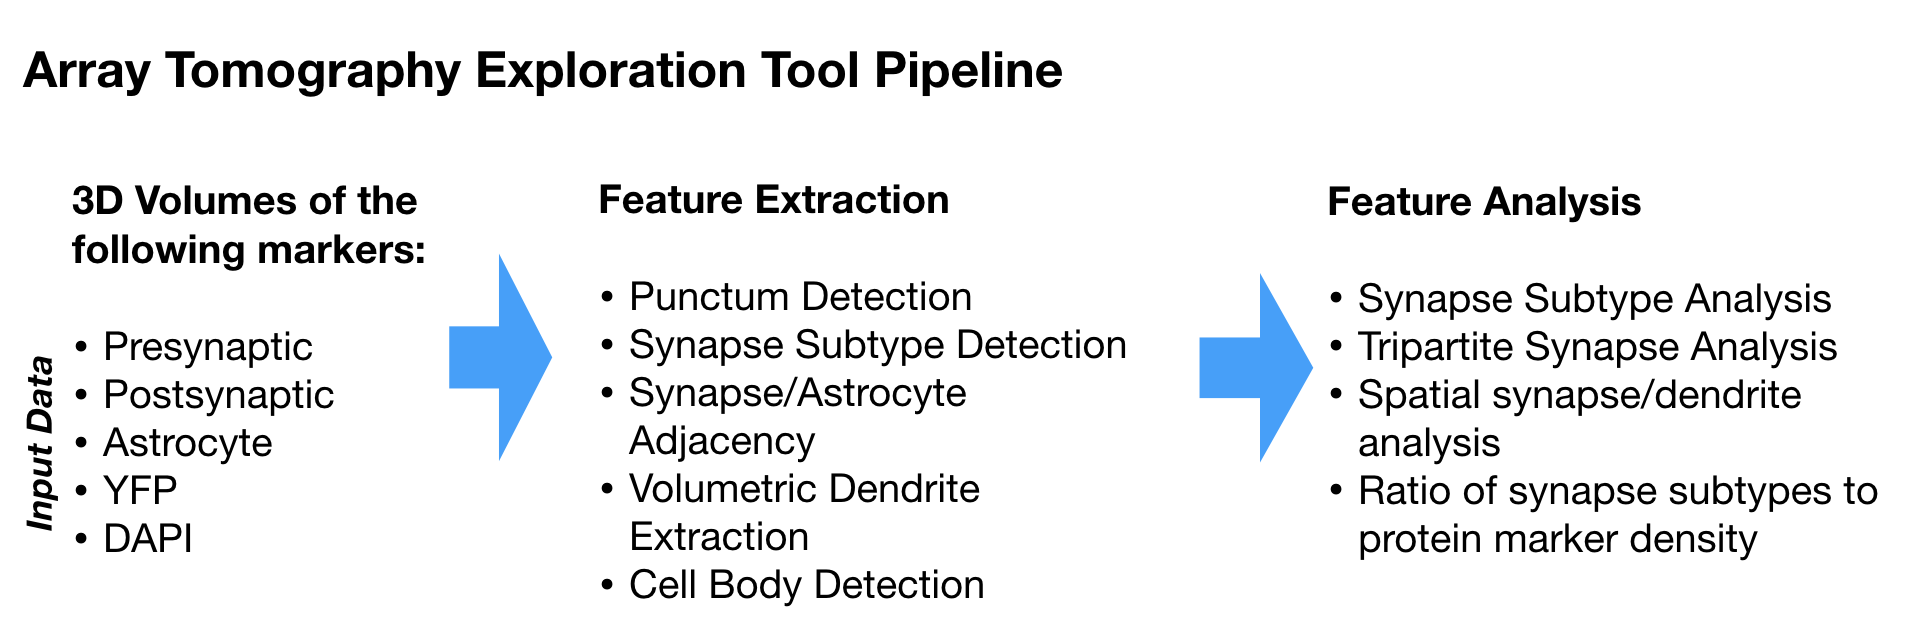
\includegraphics[width=0.7\textwidth]{figs/atetpipeline}
\caption{\textit{Pipeline of the ATET process.  Individual parts are highlighted below}}
\end{figure}

\end{block}


\begin{columns}[t]  % align column content at top

\begin{column}{\onecolwid}


\begin{block}{Synapse Detection}
\begin{figure}
\centering
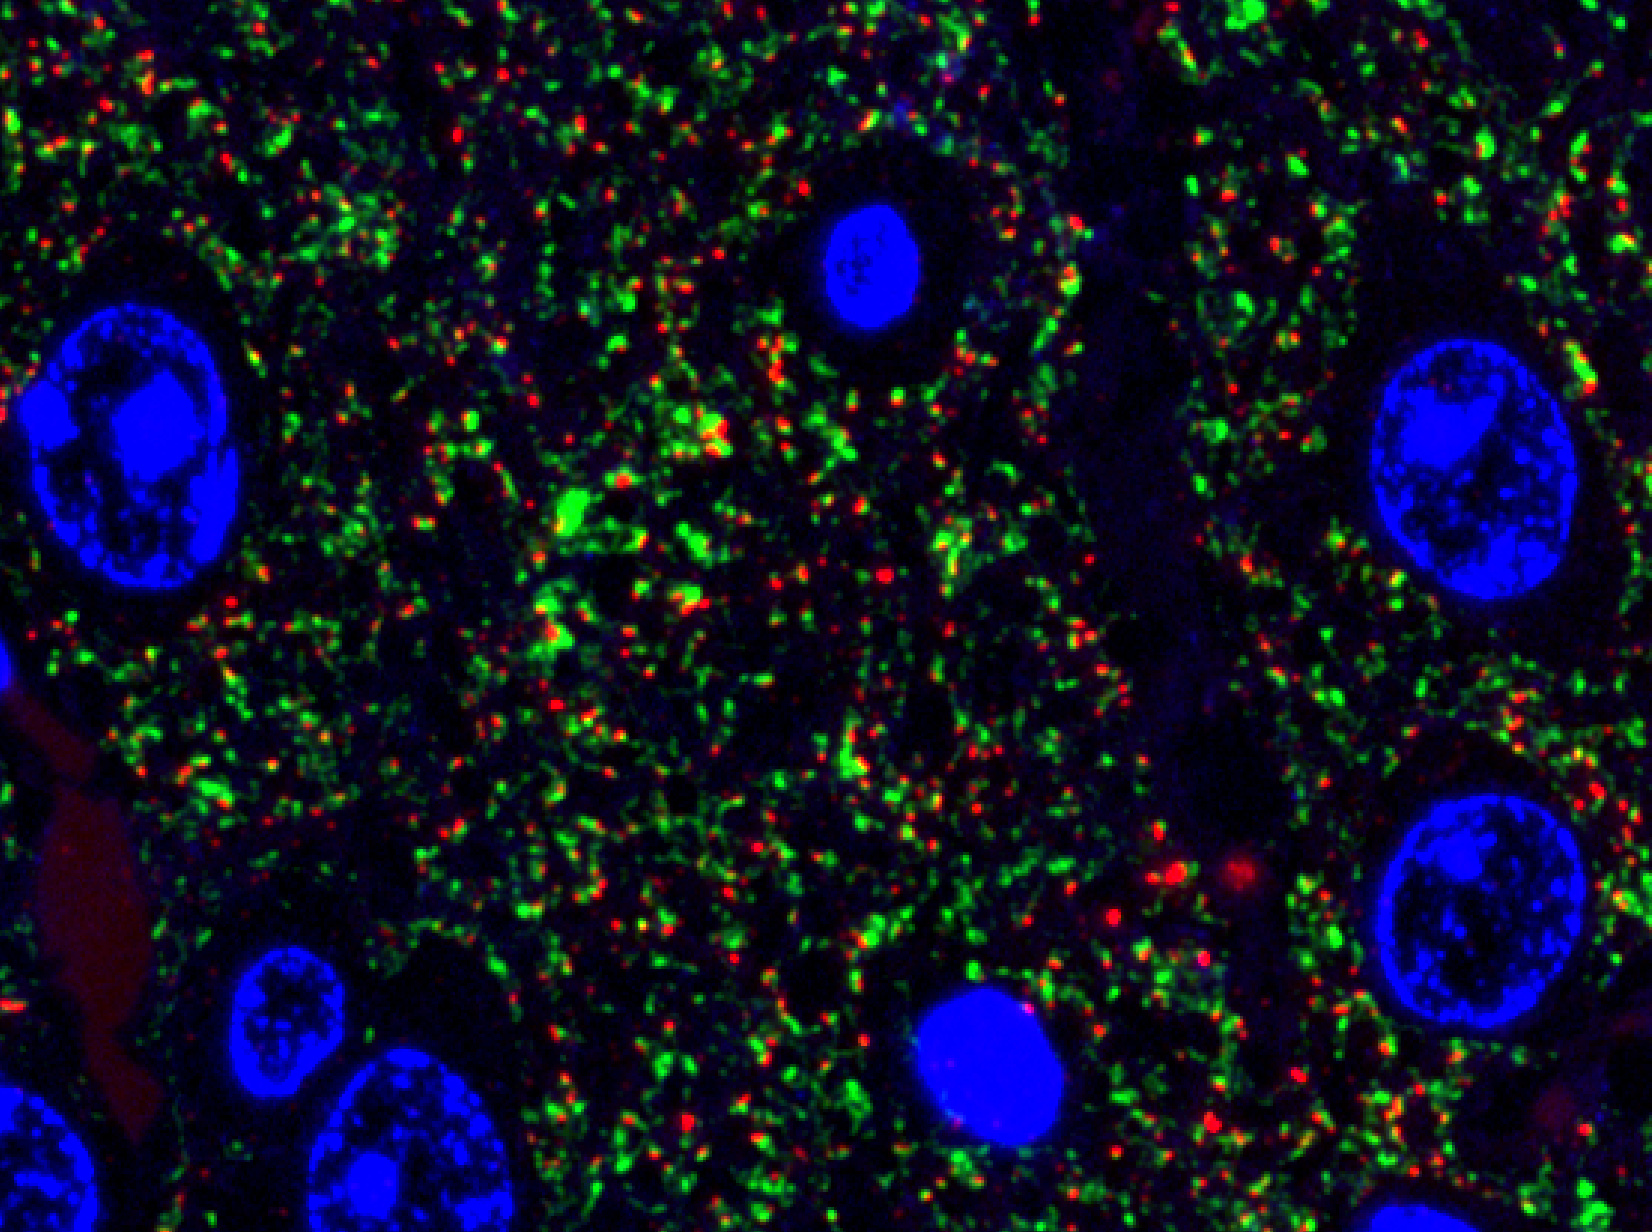
\includegraphics[width=0.8\textwidth]{figs/threechannelcutout}
\caption{\textit{Example cutout of a single slice showing three channels: red, PSD-95; green, synapsin; blue, DAPI}}
\end{figure}

\begin{figure}
\centering
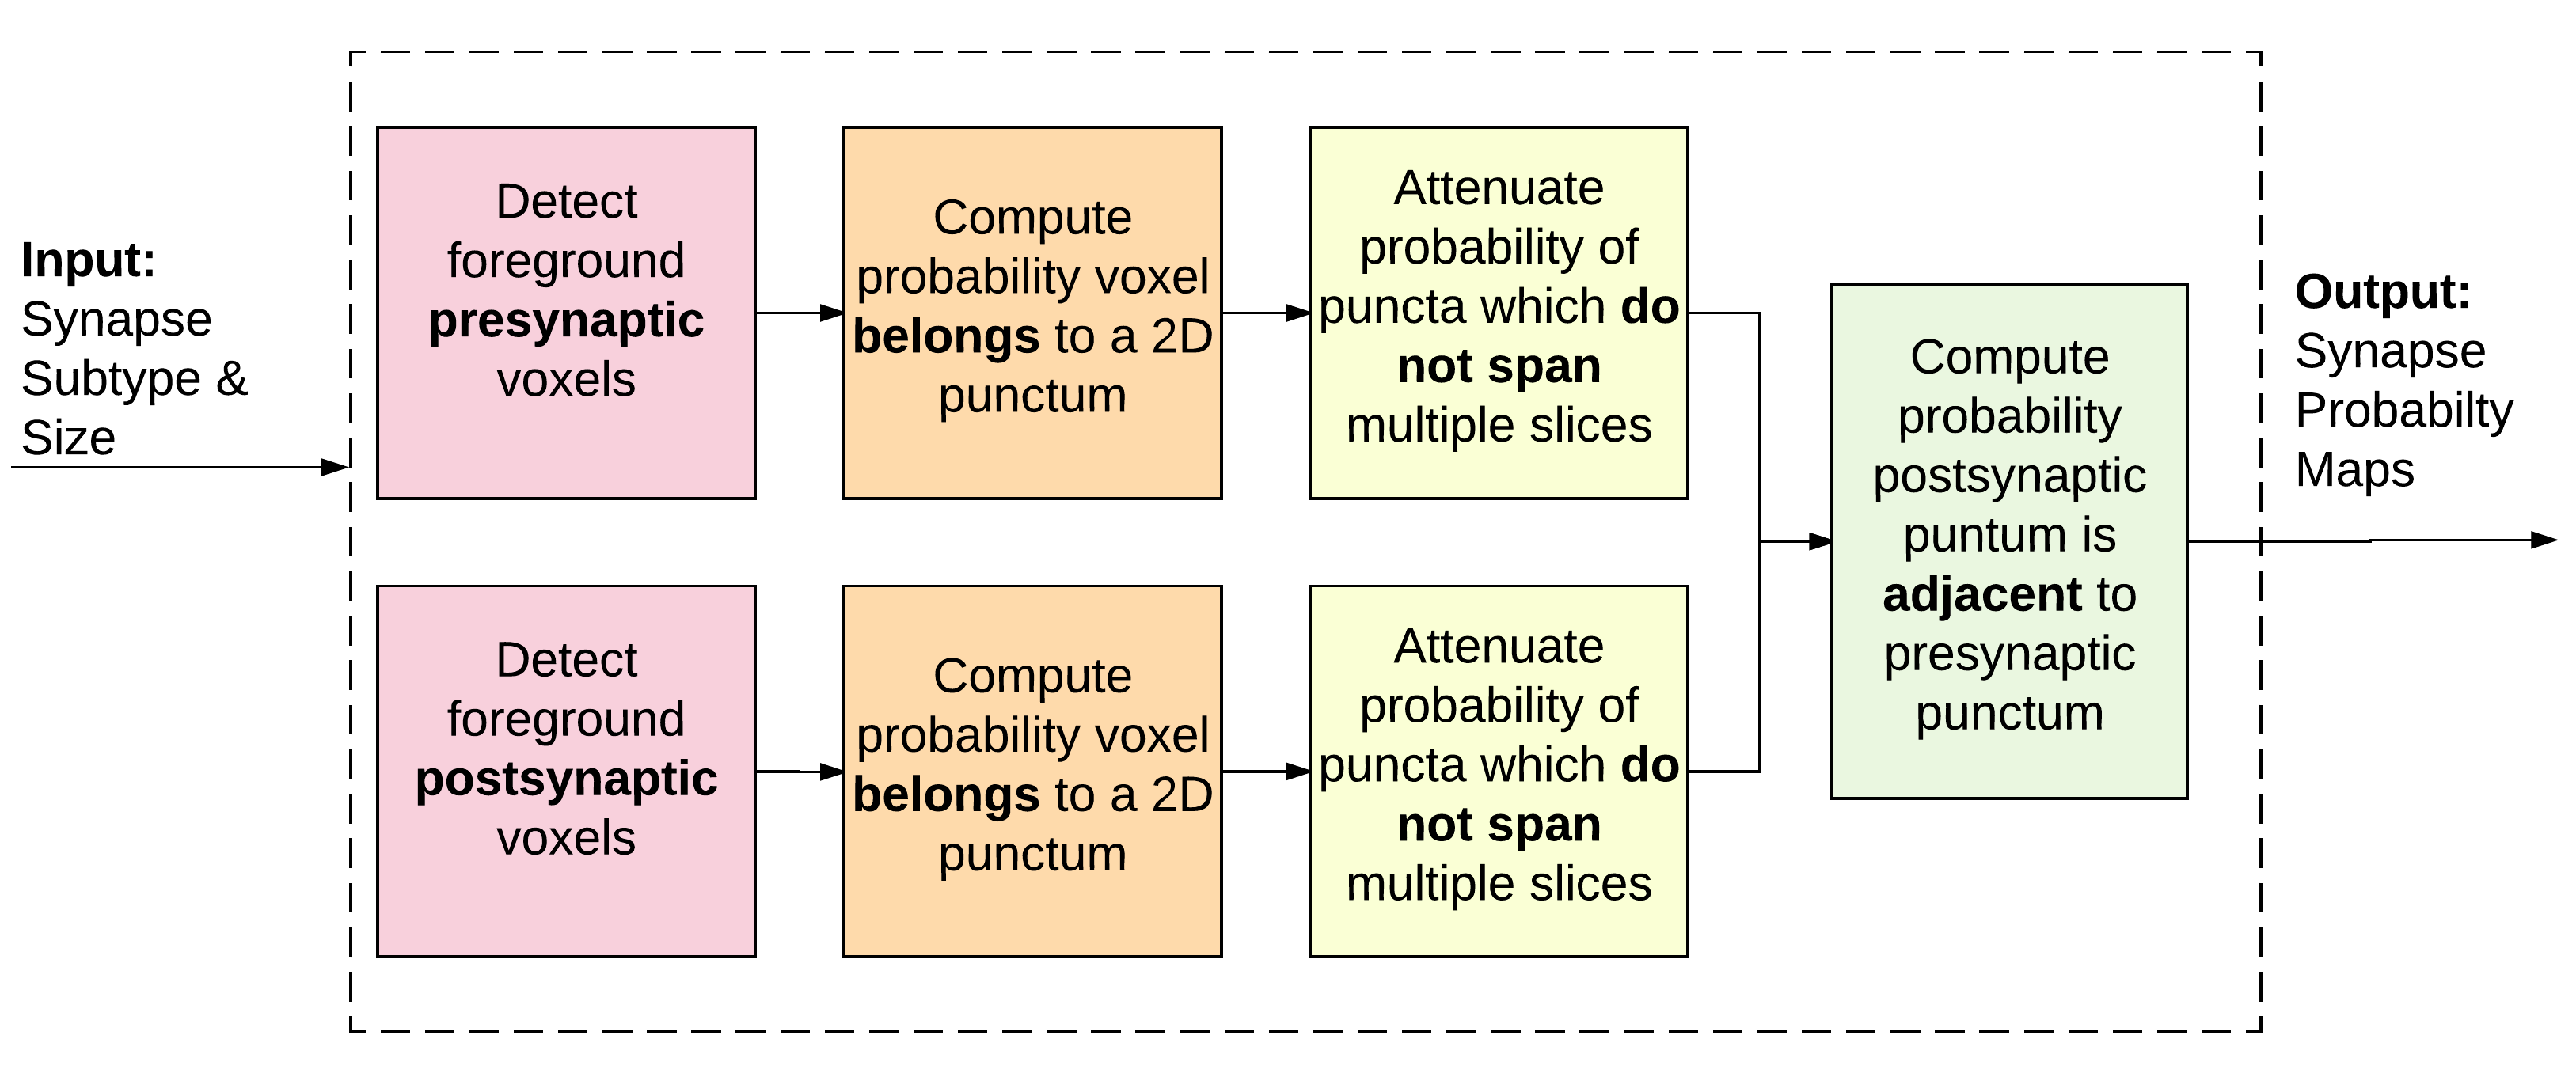
\includegraphics[width=1\textwidth]{figs/pipeline2}
\caption{\textit{Probabilistic synapse detection pipeline}}
\end{figure}

\end{block}

 
\begin{block}{Dendrite Segmentation} 

\begin{figure}
\centering
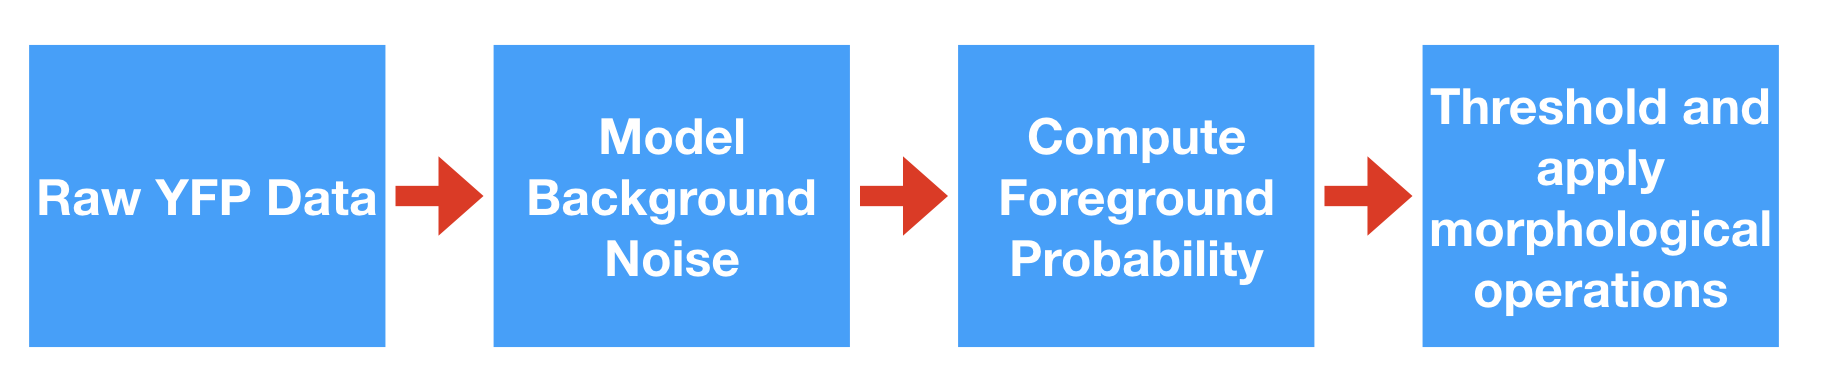
\includegraphics[width=1\textwidth]{figs/dendrite_pipeline}
\caption{\textit{Pipeline for dendrite segmentation}}
\end{figure}

A probabilistic model for the background noise, $p_{B}$, is \begin{equation} 
p_B(x,y,z) = \frac{1}{\sigma_B \sqrt{2 \pi}} \int^{\infty}_{v(x,y,z)} e^{\frac{-(t - \mu_B)^2}{2 \sigma_B^2}} d t.
\end{equation} 
Probability of a voxel associated with the foreground, $p_F$, is 
\begin{equation}
p_F(x,y,z) = 1 - p_B(x,y,z).
\end{equation}


\end{block}



\end{column}

% Third column

\begin{column}{\sepwid}\end{column}  % spacer column
\begin{column}{\onecolwid}

\begin{block}{Dendrite + Synapses} 


\begin{figure}
\centering
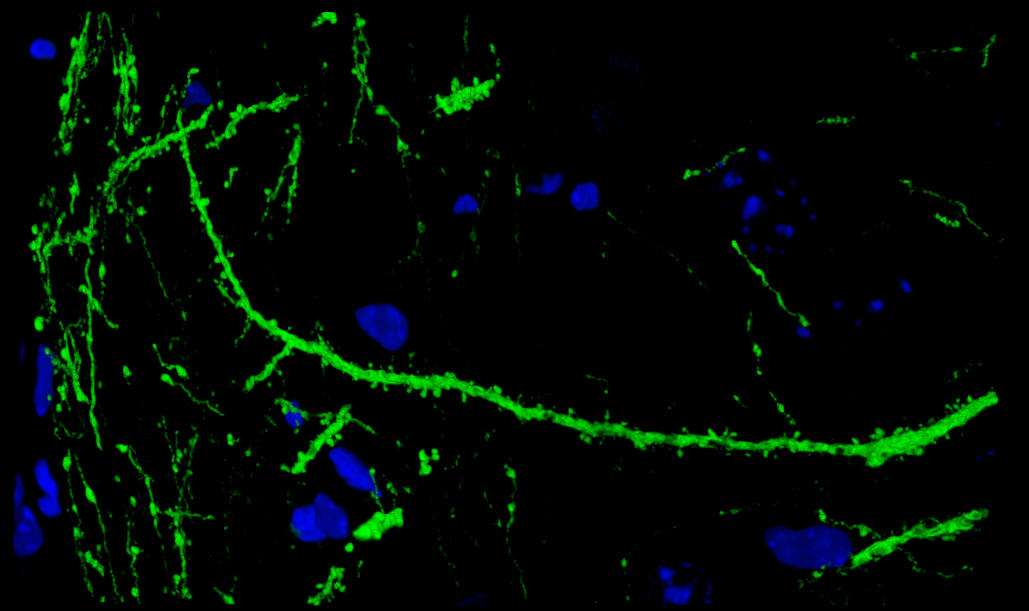
\includegraphics[width=0.8\textwidth]{figs/SnapshotDendriteR}
\caption{\textit{Maximum intensity projection of a portion of the YFP channel}}
\end{figure}

\begin{figure}
\centering
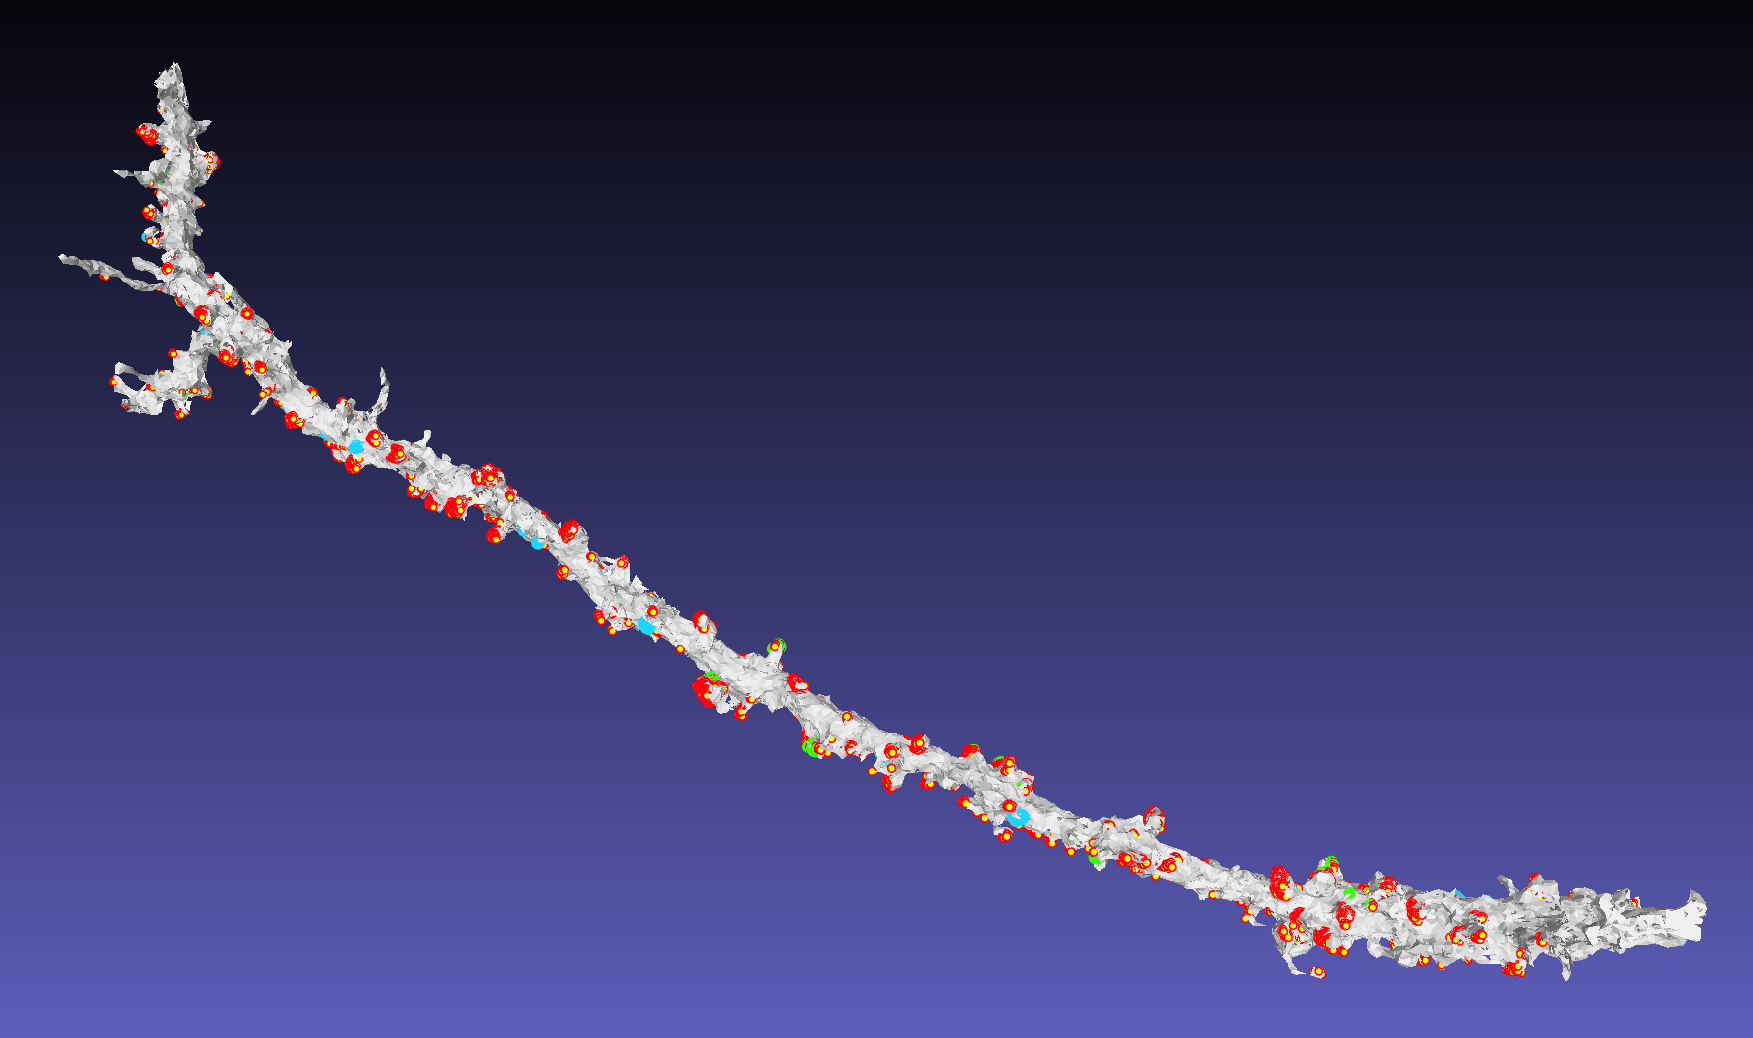
\includegraphics[width=0.8\textwidth]{figs/dendrite_allsynapses}
\caption{\textit{Segmented dendrite with various synapse subtypes marked}}
\end{figure}

\end{block}

\begin{block}{Wild-type Synapse Distribution} 
\begin{figure}
\centering
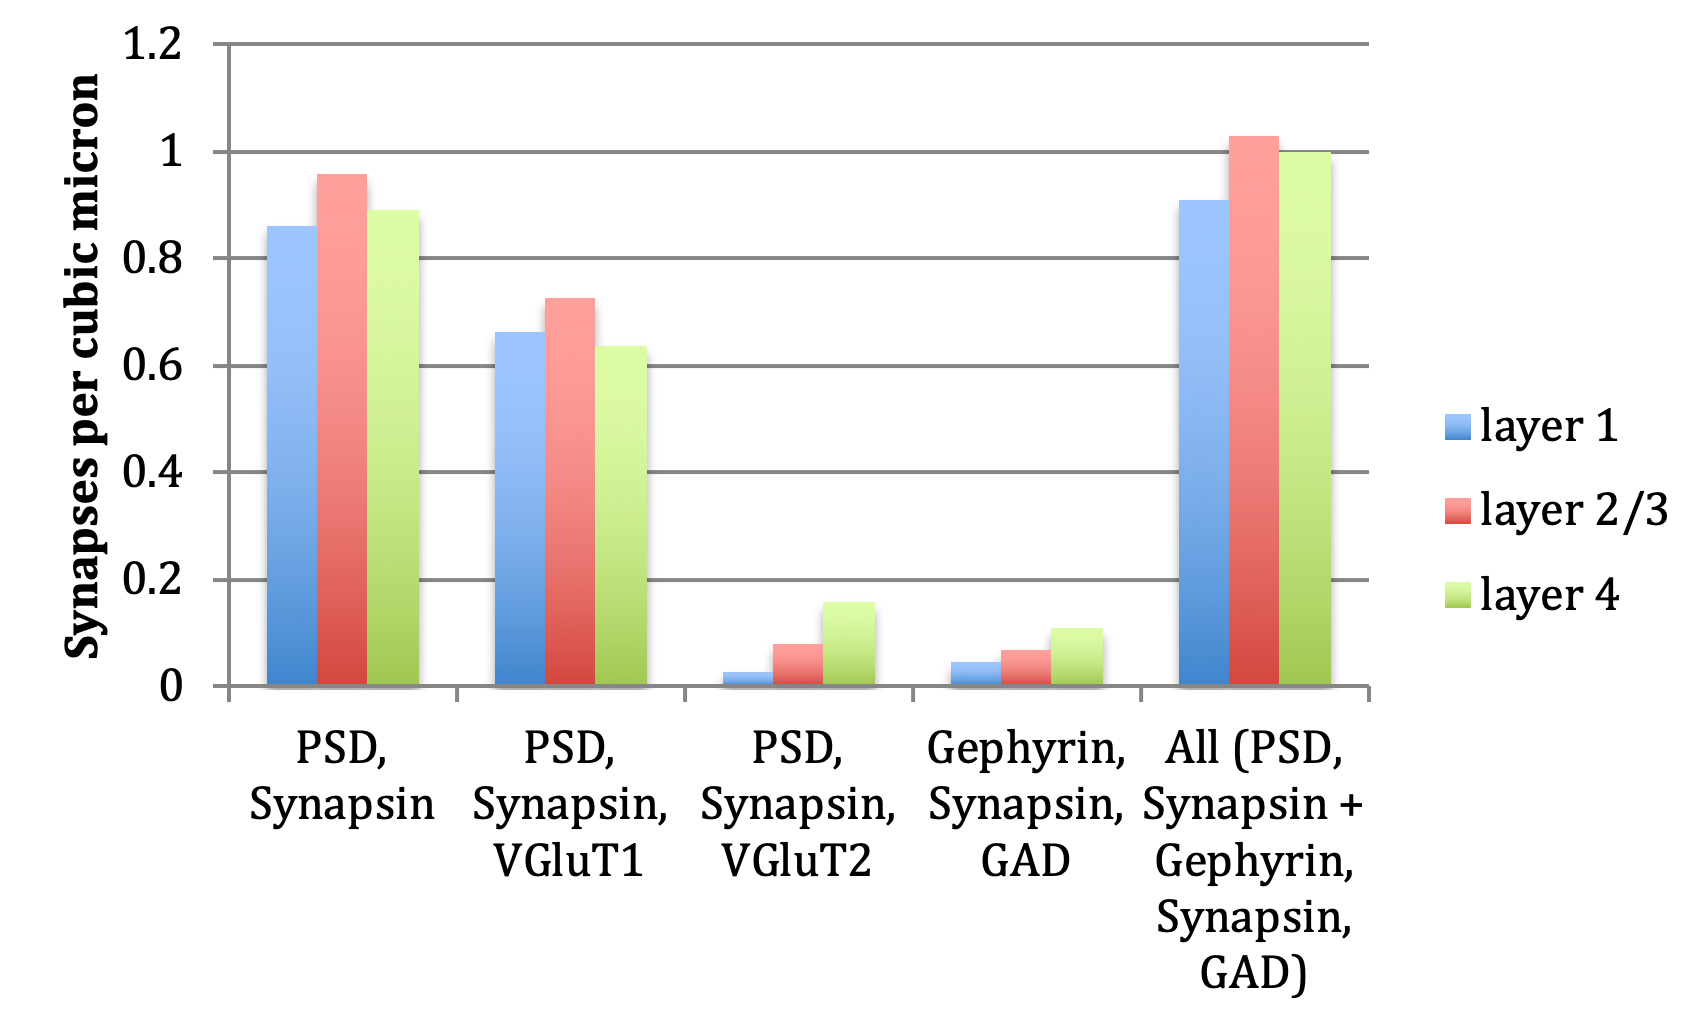
\includegraphics[width=0.7\textwidth]{figs/wildtype_synapse_counts}
\caption{\textit{Density distribution of different synapse subtypes in the upper layers of mouse barrel cortex}}
\end{figure}


\end{block} 

\begin{block}{Acknowledgments} 

\tiny{This work was supported by the National Institutes of Health (NIH-TRA 1R01NS092474), the Allen Institute for Brain Sciences (AIBS), National Science Foundation, Department of Defense, and the Information Initiative at Duke University.}
\end{block} 



\end{column}

\end{columns} 

\end{column} 

% Fourth column
\begin{column}{\sepwid}\end{column}  % spacer column
\begin{column}{\onecolwid}

\begin{block}{FMR1 Knockout Mice Analysis} 



\begin{table}
\centering
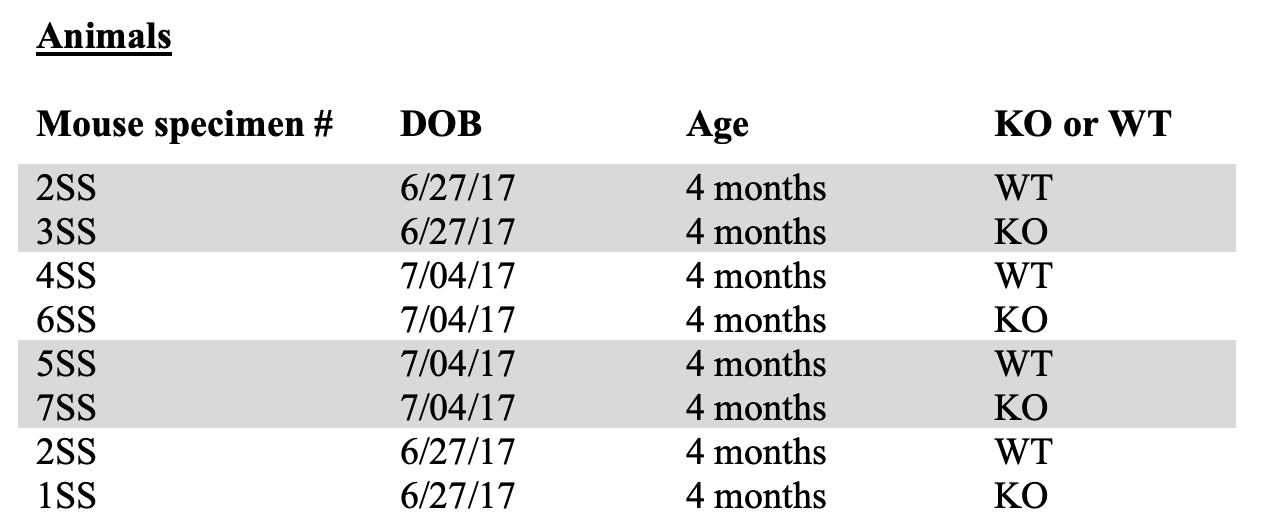
\includegraphics[width=0.8\textwidth]{figs/animal_table}
\caption{\textit{Mice used for this experiment}.  }
\end{table}

\begin{table}
\centering
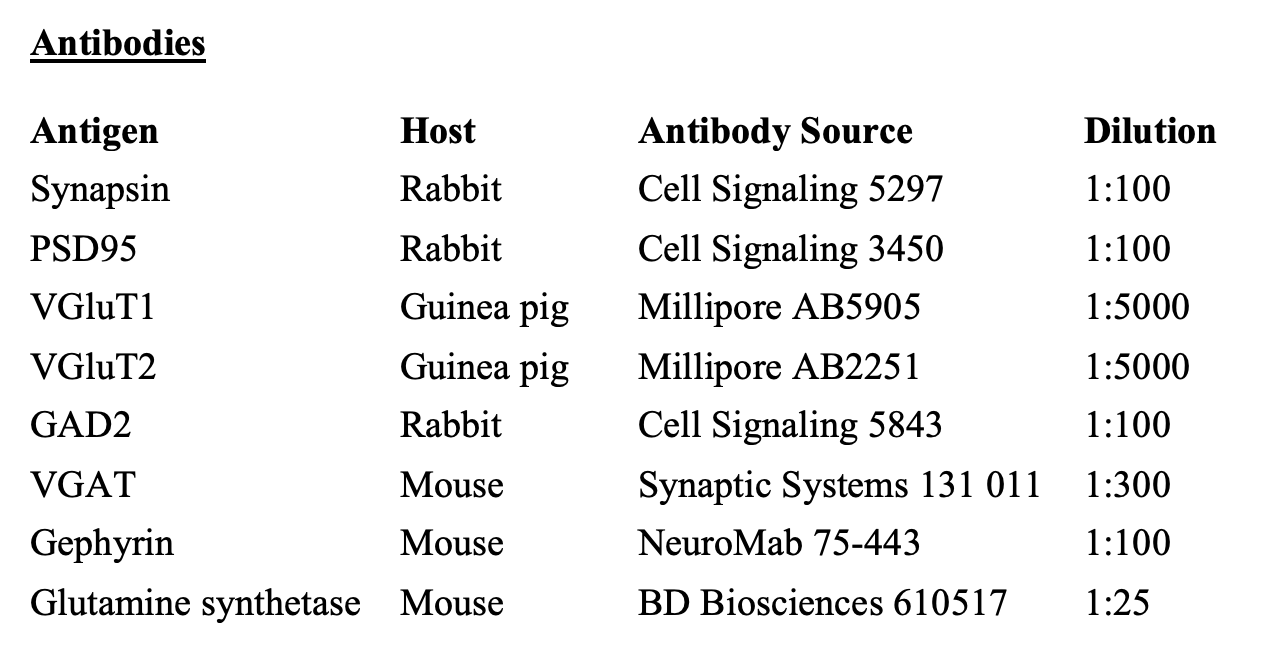
\includegraphics[width=0.8\textwidth]{figs/antibody_table}
\caption{\textit{Anitbodies used for this experiment}.  }
\end{table}


%\textbf{Synapse subtype definitions:}
%\begin{itemize}
%\small{
%\item All excitatory synapses: Synapsin + PSD95
%\item VGluT1 excitatory synapses: Synapsin + VGluT1 + PSD95
%\item VGluT2 excitatory synapses: Synapsin + VGluT2 + PSD95
%\item Inhibitory synapses: Synapsin + GAD2 + Gephyrin
%\item Astrocytic presence: as above + Glutamine synthetase}
%\end{itemize}

Density changes were calculated as $((KO-WT)/WT)*100$.  `Small synapse' refers to synapses whose puncta only span a single slice of data. 
\begin{figure}
\centering
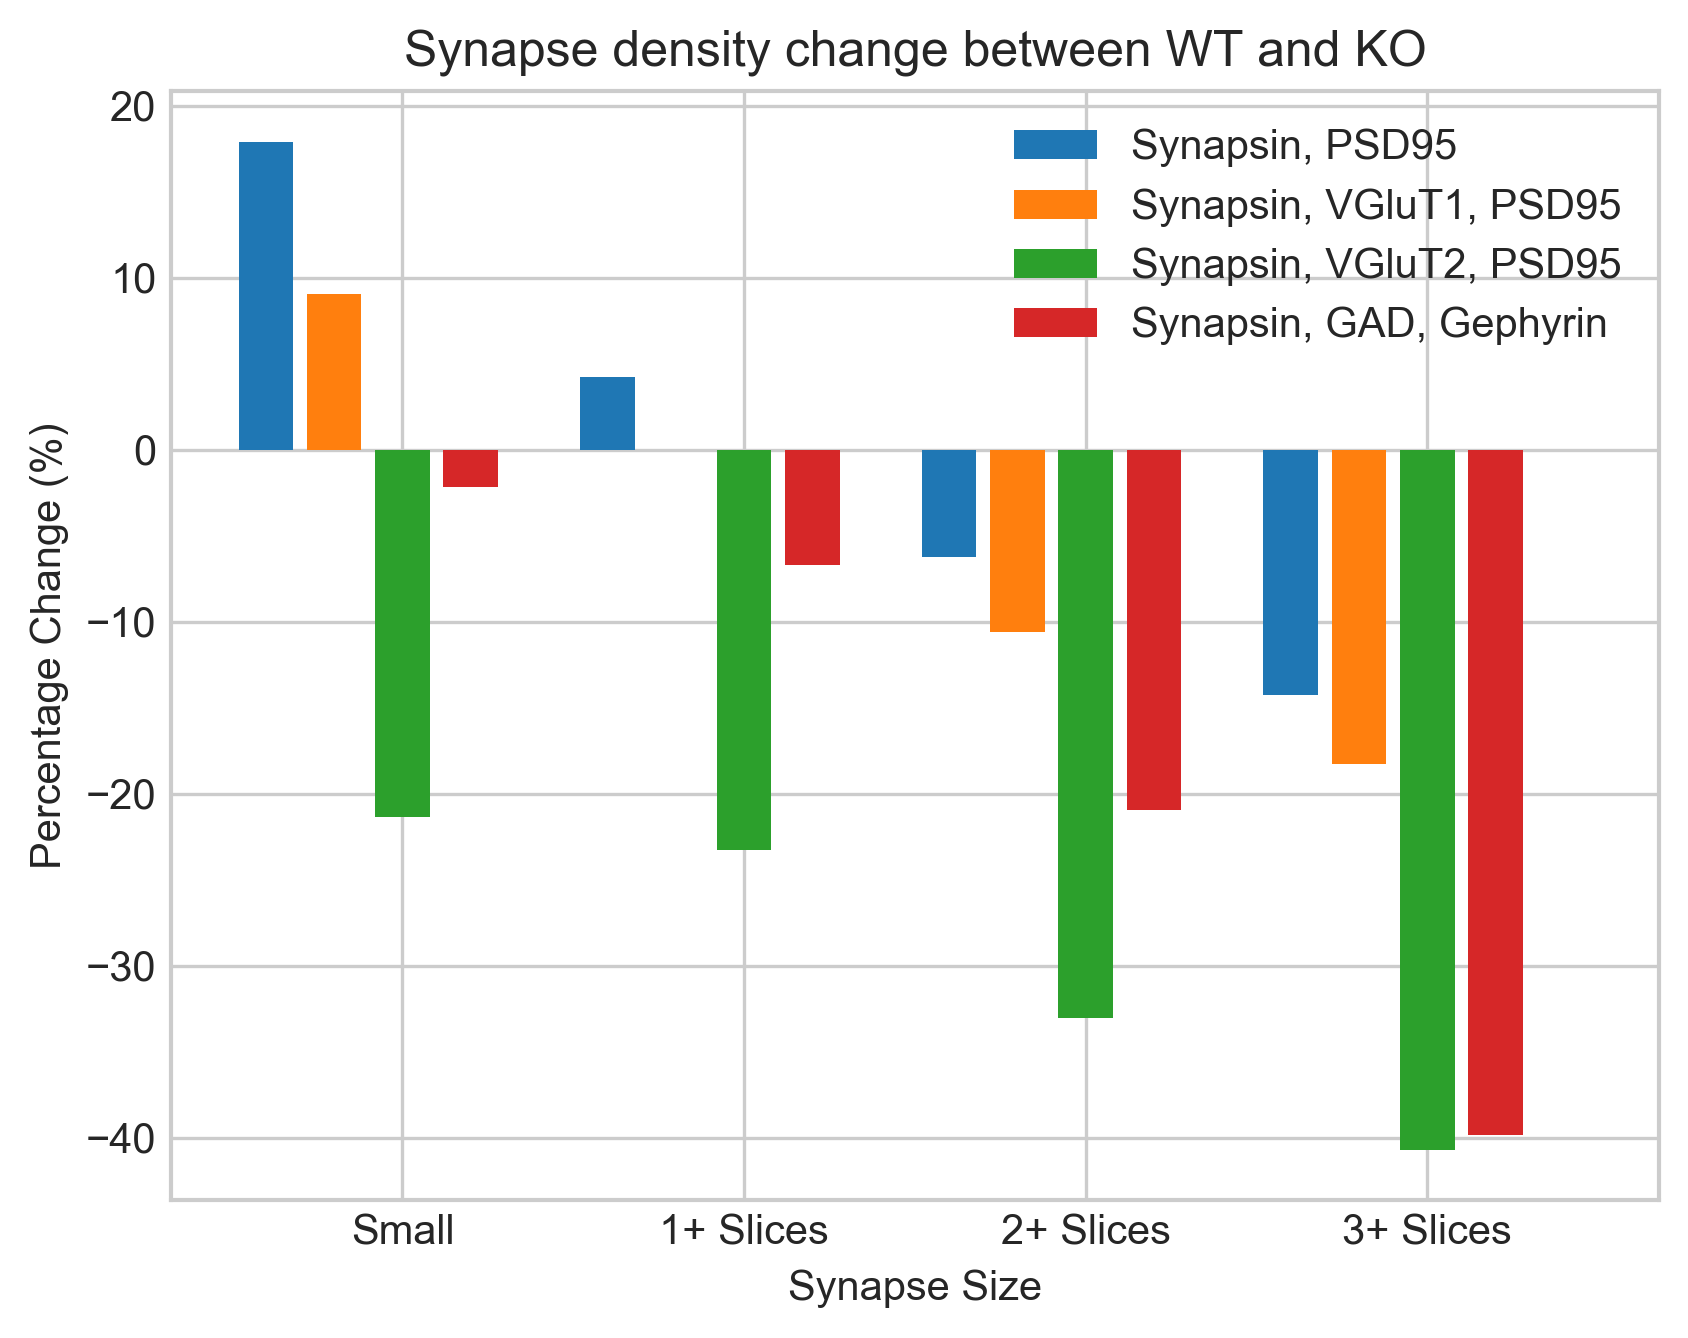
\includegraphics[width=0.8\textwidth]{figs/Synapse_Density_Change}
\caption{\textit{Synapse density change}.  Plot showing the percent change in synapse density between the wild type and knockout mice }
\end{figure}


\begin{figure}
\centering
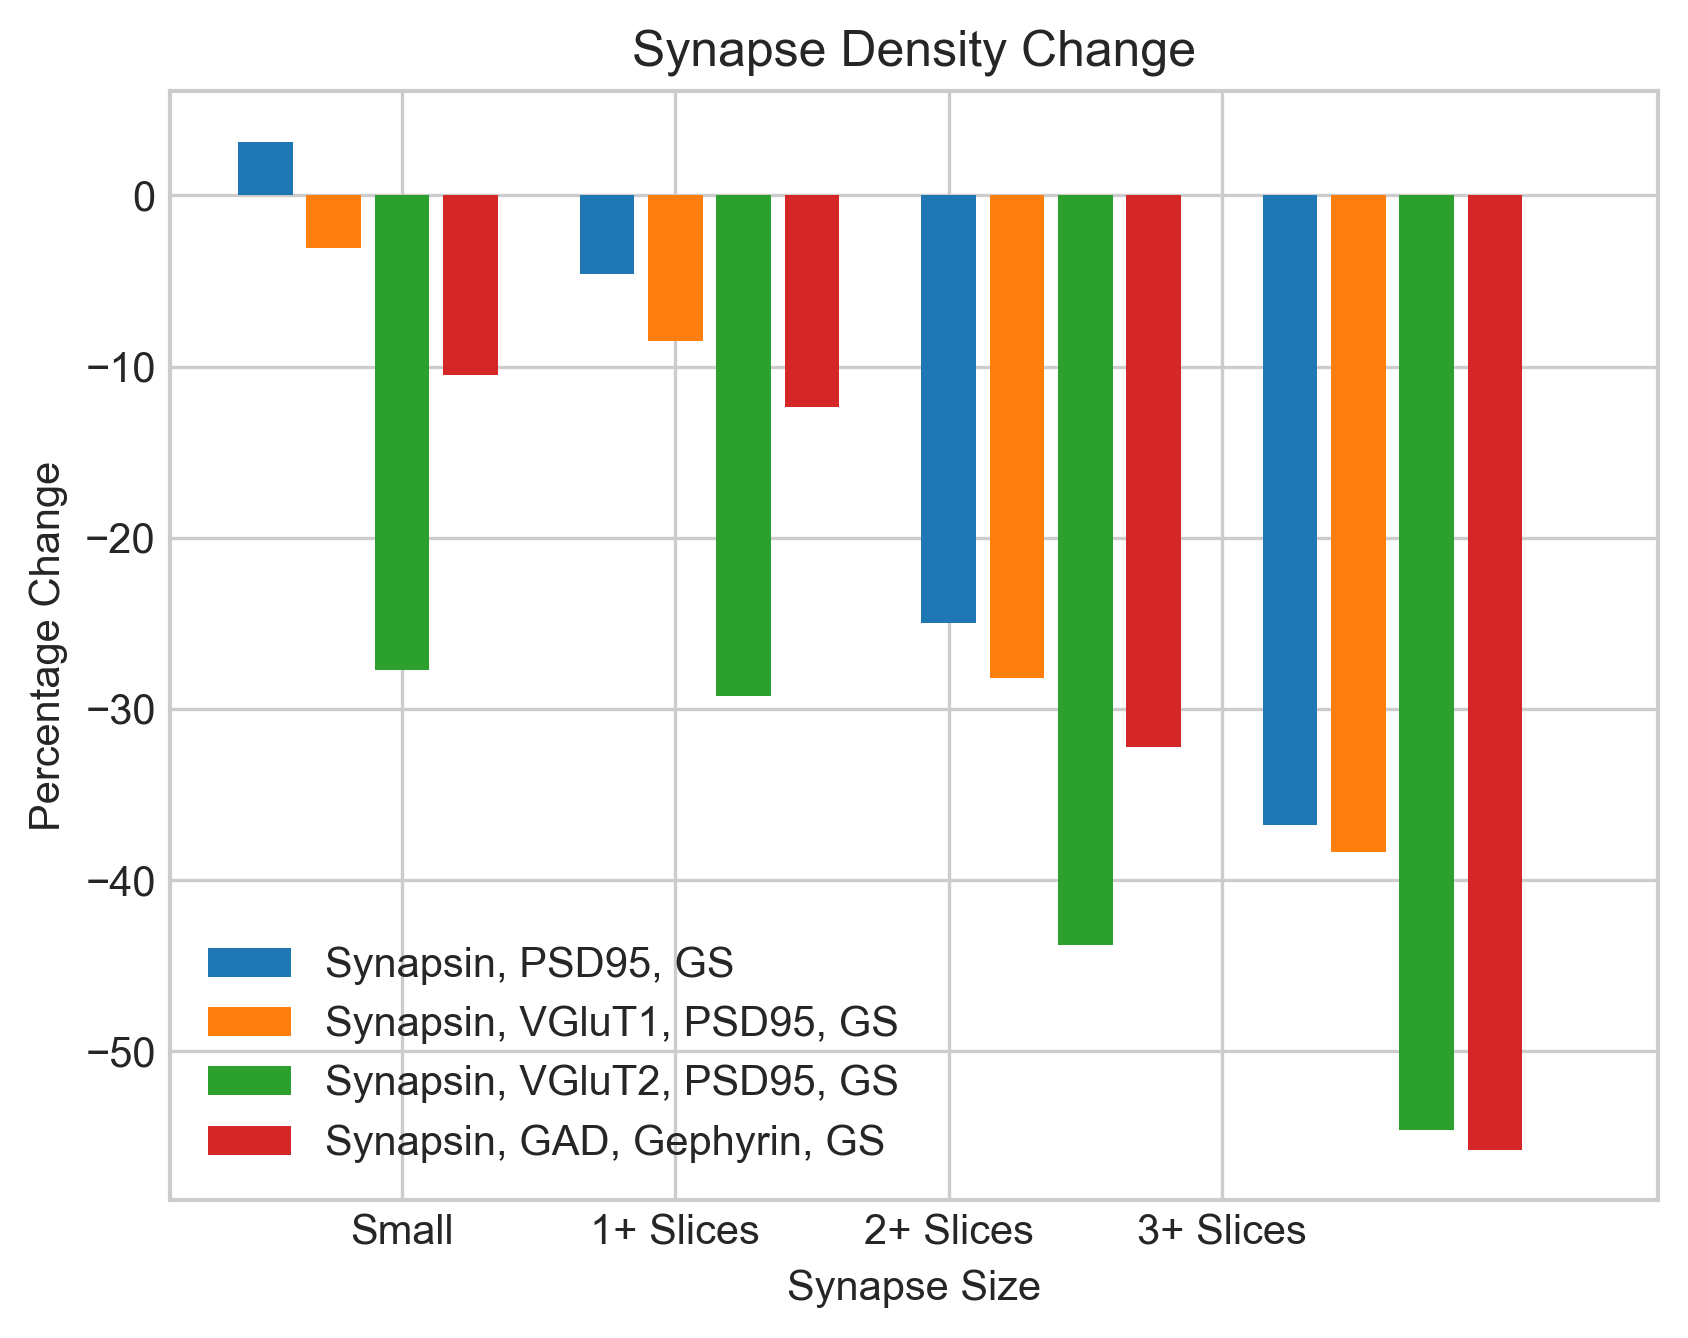
\includegraphics[width=0.8\textwidth]{figs/AstroSynapse_Density_Change}
\caption{\textit{Glial coverage change} This plot shows the percentage change in synapses that have an associated astrocytic marker between the wild type and knockout mice, for four different synapse subtypes}
\end{figure}




\end{block} 



\vspace{-0.05in}

\end{column}


\end{columns}
\end{frame}
\end{document}
